\subsection{Procesamiento}

Para generar el conjunto de datos de entrenamiento para la red se tomaron en cuenta restricciones sobre el brazo robótico a controlar y los servomotores posicionales a los que se envían las instrucciones.

El tipo de brazo robótico a controlar tiene un diseño antropomórfico, lo que significa que se compone de articulaciones unidas entre sí; además es de dos grados de libertad, lo que implica que tiene exactamente dos articulaciones. Como lo que interesa es controlar la posición (y no la orientación), se restringió la cantidad de grados de libertad del brazo robótico a uno en cada unión; esto significa que en la unión de la base existe un grado de libertad, y el otro grado de libertad se encuentra en la unión entre la primera y la segunda articulación. Además, ambos grados de libertad se mueven de arriba hacia abajo. Para alcanzar todas las posiciones posibles en el espacio, existe un grado de libertad adicional en la base que rota el brazo robótico alrededor de su eje. La Figura \ref{fig:tipobrazo} muestra un ejemplo de un brazo robótico que cumple con estas restricciones.

\begin{figure}[htb]
	\centering
	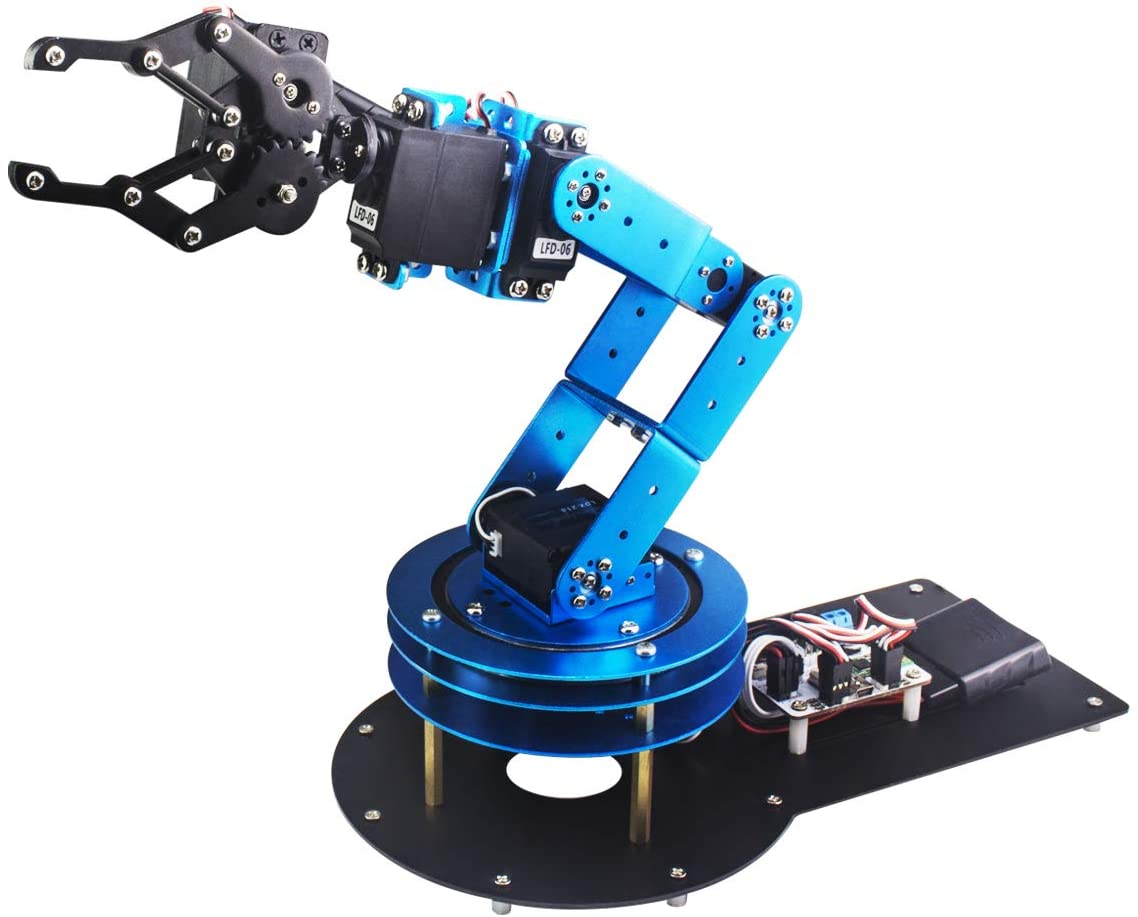
\includegraphics[scale=0.2]{tipobrazo.jpg}
	\caption{Brazo robótico de 2 DoF que cumple las restricciones impuestas}
	\label{fig:tipobrazo}
\end{figure}

El brazo robótico tiene la base en el suelo; esto significa que se puede mover dentro y en el contorno curvo de la mitad de una esfera con centro en la base del robot y de radio igual a la longitud del robot. Los servomotores posicionales solo pueden moverse en ángulos discretos, en particular, enteros. Esto significa que pueden alcanzar 180 posiciones. Además, muchas posiciones finales son lo suficientemente cercanas entre sí como para considerar que se aproximan a la misma posición.  Para determinar la proximidad de las posiciones, se aplicó el siguiente criterio con distancia Euclidiana entre dos posiciones. Si $P_1 = (x_1, y_1, z_1)$ es un punto en el espacio tal que sus coordenadas son valores enteros y $P_2 = (x_2, y_2, z_2)$ es cualquier otro punto:

\begin{equation}
	d(P_1, P_2) = \sqrt{(x_2 - x_1)^2 + (y_2 - y_1)^2 + (z_2 - z_1)^2} <= \frac{\sqrt{2}}{2} \approx 0.707
\end{equation}

De este modo, se considera que aquellos puntos que tienen a lo más 0,707 cm de distancia euclidiana entre ellos llegan a la misma posición. Para el caso en el que una de las coordenadas del punto $P_2$ sea entera, su distancia euclidiana al punto $P_1$ más cercano será menor que o igual a 0,5 cm, de modo que el criterio se reducirá a ese valor máximo. Si las posiciones alcanzables son como el punto $P_1$ antes descrito, esto significa que las posiciones alcanzables dentro del volumen de la semiesfera donde se puede mover el brazo robótico se reducen, lo que optimiza la determinación de la posición final. Note que la imprecisión es a lo más de 0.707 cm. 